\documentclass[twoside,openright,a4paper,11pt,french]{article}
\usepackage[utf8]{inputenc}
\usepackage[french]{babel}
\usepackage[T1]{fontenc}
\usepackage{emptypage}
\usepackage{amsmath}

% Utilisation d'url
\usepackage{url}
\urlstyle{sf}

% Utilisation d'images, stockées dans le répertoire ./pics/
\usepackage{graphicx}
\graphicspath{pics/}

% Définition des marges
\usepackage{geometry}
\geometry{
  left=25mm,
  right=25mm,
  top=25mm,
  bottom=25mm,
  foot=15mm
}
\usepackage{listings}
\usepackage{color}

\definecolor{gray}{rgb}{0.8,0.8,0.8}

\begin{document}

\pagestyle{plain}
\setlength{\parindent}{0pt}
% La page de garde
\thispagestyle{empty}

\begin{center}
       \noindent
       
\includegraphics[height=2.5cm]{./pics/uds.eps}       
       
       \vfill\vfill

    {\large \textsc{Licence 3 de Sciences, mention Informatique}}

    \bigskip\bigskip

    {\large \textsc{Programmation Orientée Objet 2 }}

    \vfill\vfill

% Titre du document
    {\huge \sc
      \begin{center} 
        Rapport sur le projet: \\
        détection des bords et vectorisation
      \end{center}}

    \vfill\vfill

    {\large Présenté par}

\medskip

% Identité des auteurs
    {\large Victor \textsc{Constans}}\\
    {\large Luigi  \textsc{Coniglio}}\\
\bigskip

\end{center}



% La table des matières
\parskip=0pt
\tableofcontents


\vspace{5cm}

%Start content

\section{Fichiers rendus et usage}
\subsection{Contenu du rapport}
L'objectif de ce rapport est d'abord celui d'illustrer la structure du
programme. Pour accelerer/simplifier l'utilisation du travail rendu, la partie
initiale de ce rapport décrit le contenu des fichiers et leur usage.

\subsection{Contenu de l'archive}
Après avoir ouvert l'archive {\it constans\_coniglio\_luigi.tar.gz} vous
trouverez les fichiers et repertoires suivants:
\smallbreak
\begin{itemize}
\item Ce rapport
\item Les fichier {\bf javimy.java} est le point d'entre du programme
\item Le repertoire {\bf gui} contiens tous les fichiers to du programme relatifs
      a l'interface graphique
\item Le repertoire {\bf filters} contient un package incluant tous les filtres 
      implemente dans la candre de ce projet
\item Le repertoire {\bf vectorization} contients la partie du programme dedie a
      la vectorisation d'une image
\end{itemize}

\bigbreak

\subsection{Usage}
Compilez le programme par le biais de la commande 
\colorbox{gray}{\lstinline[basicstyle=\ttfamily\color{black}]| javac javimy.java |}
Une fois termine la création des fichiers {\it .class} vous etes pret
a utiliser ce magnifigue logiciel: 
\colorbox{gray}{\lstinline[basicstyle=\ttfamily\color{black}]| java javimy |},

\vspace{1cm}
A l'execution il vous serait presente une interface graphique que vous
permettra de facon assez intuitive d'acceder aux different functions
du programme:

\begin{center}
% TODO image GUI %
\end{center}

\newpage 

\section{Filtres}
\label{sec:filtres}

\subsection{Sobel, Prewitt, Roberts, etc...}
Description du principe de fonctionnement avec quelque image/example

\subsection{Canny}

\subsection{Gauss}
Description du principe de fonctionnement avec quelque image/example

\subsection{Segmentation}
La segmentation a l'objectif de partitionner un image en sections
(ensembles de pixels) sur la base de leurs propriete (couleurs,
intensite, ...). Dans le menu des filtres vous trouverez un bouton qui
va vous permet de realiser cette type de operation sur les couleurs
d'une image. 

L'algoritme utilise pour segmenter l'image est inspire du
partitionnement en {\it K-moyennes} (ou {\it k-means clustering} en
anglais). Ce type de partitionnement consiste a selectioner K couleurs
et assigner chaque pixel de l'image a le plus proche de ces couleurs.

\begin{figure}[h]
\centering
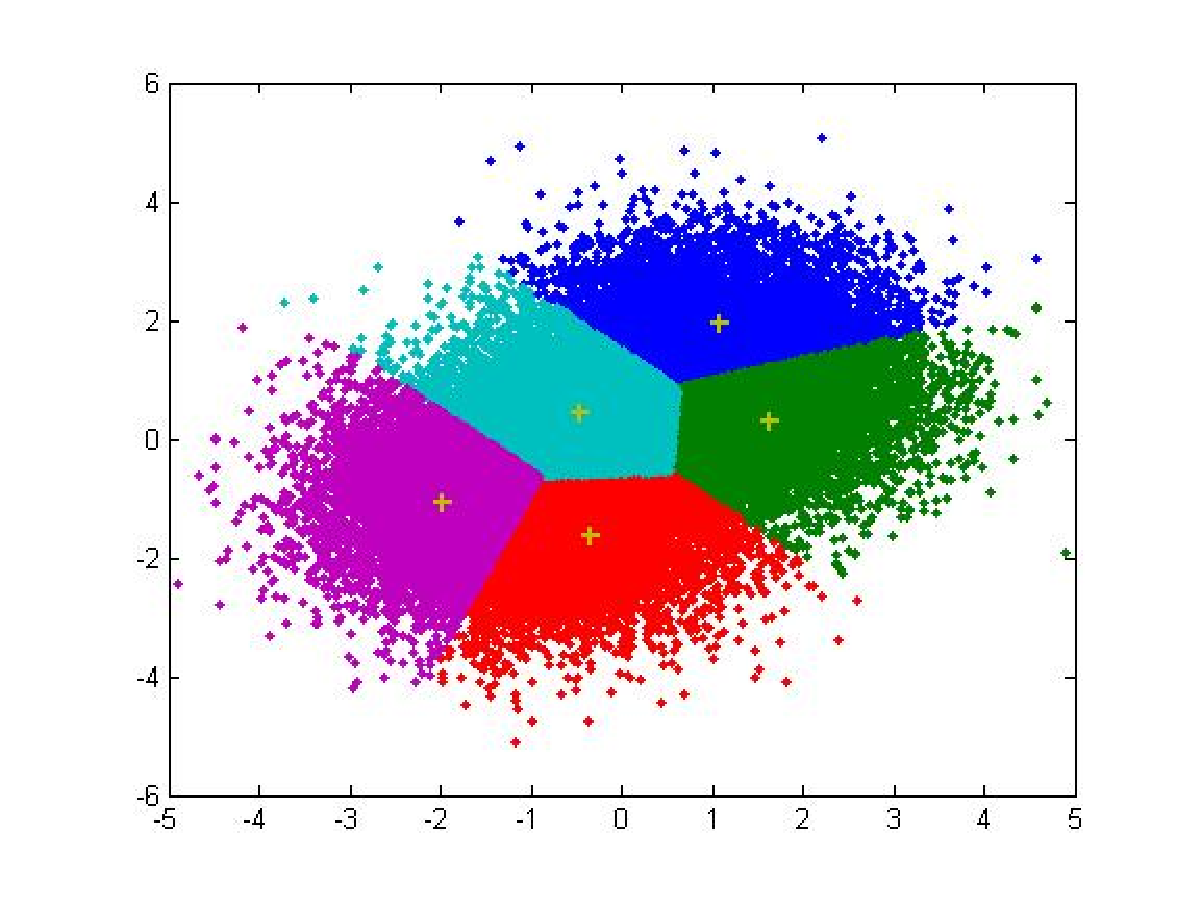
\includegraphics[width=8cm]{./pics/kmeans.eps}
\caption{Agrégation des pixels selon la plus courte distance avec les
K-moyennes (ici K = 5)}
\label{fig:routcidr}
\end{figure}

Les K couleurs sont apres modifie pour minimiser les distances avec
les pixel de l'image, les groupement par couleurs refait et ainsi de
suite jusq'a quand les K couleurs et le partitionnement des pixels
convergent. 

\subsection{Cluster-edges}
Cet filtre s'inscrit dans l'ensemble des filtres de detections des
bords. La particularite de ce filtre par rapport aux autres filtre de
detection des contours est que il n'effectue pas une simple detection
des bords mais, plus precisement, il determine les limites entre
differents zones de couleurs. 
Les limites entre deux zones de couleurs sont represente par des
chemin colore. A chaque bord correspond un chemin d'un couleur
different \cite{url-novelvect}.

Le premiere etape de l'algoritme consiste a segmenter l'image en
different zones de couleurs.

\begin{figure}[h]
\centering
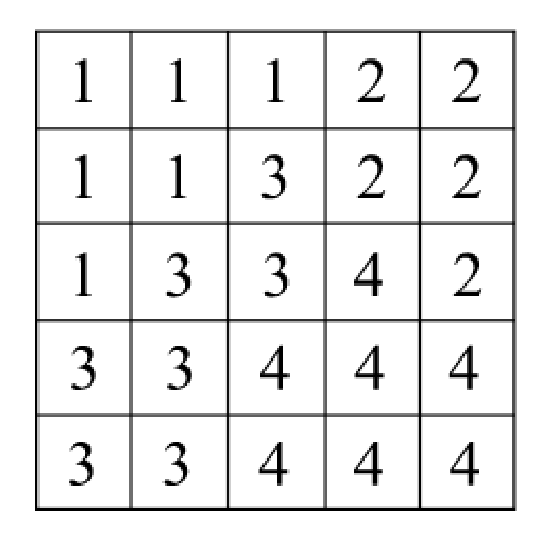
\includegraphics[width=3.5cm]{./pics/cluster-edges1.eps}
\caption{Segmentation, chaque nombre represente un couleur different}
\label{fig:routcidr}
\end{figure}

Une fois termine la segmentation on procede a la generation de
sub-pixels entre chaque pixel de l'image originaire. Chaque sub pixel
est rempli en raison du couleur des pixel autour de lui.

\begin{figure}[h]
\centering
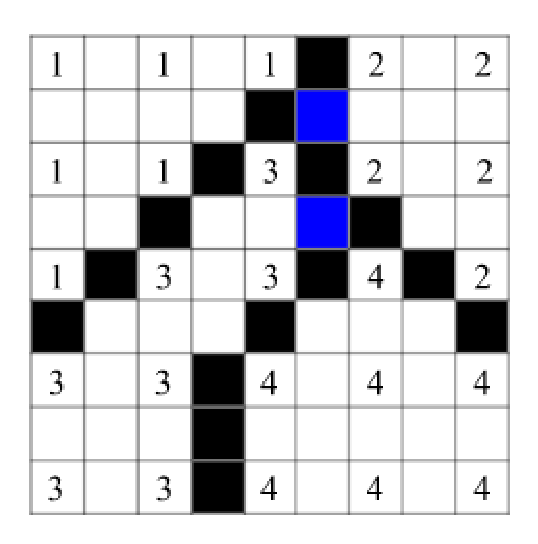
\includegraphics[width=3.5cm]{./pics/cluster-edges2.eps}
\caption{Les bords sont les subpixel ayant comme voisins des pixel de
couleur different}
\label{fig:routcidr}
\end{figure}

\newpage

\section{Vectorisation} 
Le programme permet d'exporter une image sous la forme d'un fichier
{\it .svg}. La conversion d'une image dans le format SVG ({\it
Scalable Vector Graphics}) suive un processus assenz complex que vaut
la peine d'etre presente.

Si la plupart des formats representant une image en utilisant un 
mappage plus ou moin complex des pixels, un format d'image vectorielle
permet de representer une image comme etant un ensemble de formes
egendre par des vecteurs. Vectoriser une image constiste a traduire
l'ensembles des pixels d'une image en vecteurs (formes geometriques,
chemins, courbes, etc ...).

L'algorithme utilise dans le candre de ce projet pour vectoriser une
image peut etre resume dans les etapes suivantes:   

\smallbreak
\begin{itemize}
\item Segmentation de l'image
\item Detection des contours et extraction des bords
\item Compression des bords
\item Construction des figures
\item Conversion au format SVG
\end{itemize}   
\bigbreak

La segmentation et la detection des contours d'une image sont effectue
en utilisant les techiques presentes dans la section
\ref{sec:filtres} de ce rapport.


\subsection{Compression des bords}
%TODO Algorithme de Douglas-Peucker %
Au moment de sa detection chaque bord est extrait comme etant une
suite continue de pixels. Bien que un telle representation soit tout a
fait utilisable dans la construction d'une image vectorielle le
resultat ne serait pas tres different de celui d'un format standard
d'image. Pour cette raison pendant le processus de vectorisation d'une
image les suites continues de pixels constituees pas les contours de
l'image doivent etre traduite par des elements geometriques plus
simples: segments, courbes, etc.. .  

Le premiere etape dans la traduction des contours consiste a en reduir
le nombre de pixels. Dans la cadre de ce projet on a decide d'utiliser
l'algoritme de Douglas-Peucker pour atteindre cet objectif
\cite{url-dougpeuck}.

L'algoritme de Douglas-Peucker est beaucoup utilise en geographie dans
et permet d'approximer les points d'un chemin en tenant compte d'un
certaine degre de liberte (parametrable).

\begin{figure}[h]
\centering

\includegraphics[width=7cm]{./pics/dp1.eps}
\caption{Le bords sont approxime avec un degree de liberte croissante}
\label{fig:routcidr}
\end{figure}

Le fait que cet algoritme soit facilement parametrable a ete un
element cle dans la choix et il permet a l'utilisateur de choisir la
precision souhaite dans la vectorisation.

Un autre element essentiel dans la choix de cet algorithme a ete le
fait que il ne change pas la position du premier et le dernier point
d'un chemin dans la compression de celui-ci. Grace a ca un chemin
(partie d'un contour) d'une image commencera et terminera toujour sur
le meme points meme apres sa compression, en assurant ainsi la
contiguite de celui ci avec les bords voisins.



\subsection{Construction des figures}
%TODO voisinage de moore %
Une fois simplifie les contours il est arrive le moment de traiters
les zones de couleurs egendre par les bords.

On peut definire une {\it figure} comme etant une section de l'image
ayant (apres segmentation) un unique couleur et egendre par un ou
la combinaison de plusieurs bords.

Le but de ce stade est de detecter toutes les {\it figures} dans l'image et
de affecter a chaque {\it figure} les bords entourant celle-ci dans le
bon ordre (sachant que un bord est partage toujours entre deux
{\it figures}).

L'algoritme pour la construction des {\it figures} consinste a parcourir
l'image a la recherche des zones de couleurs. 

\begin{lstlisting}[frame=single]  % Start your code-block
Construction figures ( image )

Pixel p
Couleur c
Figure figures[]
Pour i=0...image.hauteur faire
    initialise c tel que c != image.pixel(i,0).couleur 
    Pour j=0...image.largeur faire
        si image.pixel(i,j).couleur != c et 
           image.pixel(i,j).traite = faux

            f <- image.pixel(i,j).extrait_figure()
            figures.ajouter(f)

            Pour tout pixel b dans f faire
                image.pixel(b.y,b.x).traite <- vrai
            fin 
        fin 
    fin
fin
renvoyer figures
\end{lstlisting}


Apres avoir detecte une zone qui n'a pas encore ete traite, on procede
a examiner les voisins \underline{externes} des pixels qui delimitent
la {\it figure}.

\begin{figure}[h]
\centering
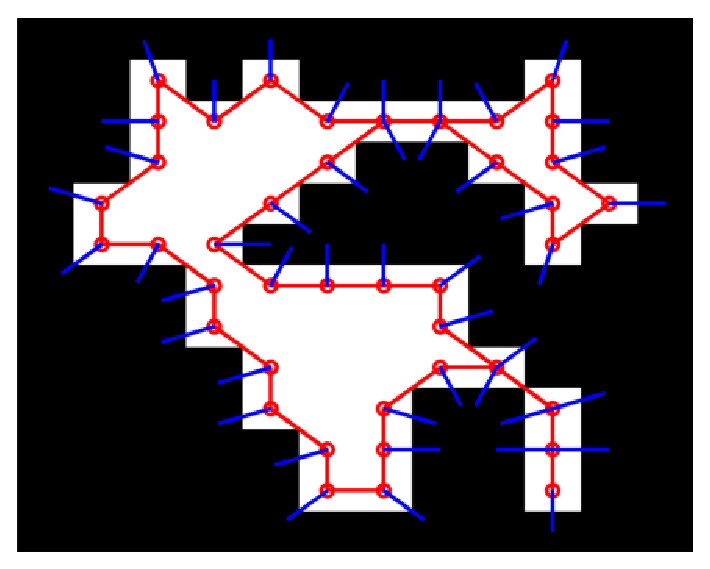
\includegraphics[width=7cm]{./pics/moore.eps}
\caption{Detection du voisinage externe d'une {\it figure}}
\label{fig:moore}
\end{figure}

Les contours d'une {\it figure} sont examine dans le sens horaire en
utilisant l'algoritme du voisinage de Moore \cite{url-moore}.




\section{Valeurs optimales}
%TODO valeurs optimales dans l'utilisation de chaque filtre%



\newpage
\addcontentsline{toc}{section}{Références}
\bibliographystyle{plain}
\bibliography{rapport}

\end{document}
